\section{Muhammad Fahmi}

\subsection{Sejarah Pyton}
Guido Van Rossum adalah orang yang menciptakan python di Scitching Mathematisch Centrum (CWI) Belanda pada wal tahun 1990-an. 
Pada nama python sendiri berasal dari nama ular yang kita tau. Guido Van Rossum seorang yang menggemarkan grub komedi inggris yang bernama Monty Python, Lalu ia menamakan ciptaannya dengan nama Python
Bahasa python terinspirasi dari bahasa pemrograman ABC. Nama python tidak berasal dari nama ular yang kita kenal. Guido merupakan penggemar grup komedi Inggris bernama Monty Python. Kemudian, ia menamakan Bahasa pemrograman ciptaannya dengan nama Python.
Pada tahun 1994, Python 1.0 dirilis, yang diikuti dengan Python 2.0 pada tahun 2000. Python 3.0 keluar pada tahun 2008.

\subsection{Instalasi Anaconda}
\begin{enumerate}
    \item Pastikan Bahwa Python telah terinstall dilaptop anda.
    \item Download File Installer Anaconda pada www.anaconda.com
    \item Install seperti biasa 
    \item Kemudian Klik I Agree
    \item Kemudian Centang yang register Anaconda as default Python, Kemudian Pilih Next
    \item Tunggu Proses Instalasi hingga selesai
    \begin{figure}[H]
		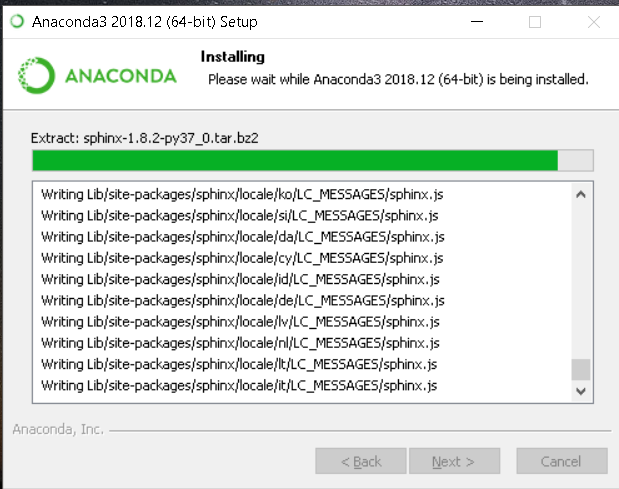
\includegraphics[width=10cm]{figures/fahmi/1.png}
		\centering
	\end{figure}

    \item Instalasi telah selesai
	 \begin{figure}[H]
		
\includegraphics[width=10cm]{figures/fahmi/2.png}
		\centering
	\end{figure}
	
\end{enumerate}
	

\subsection{Penggunaan Spider}
Spyder merupakan text editor dari anaconda dimana di tools ini bisa menjalankan perintah-perintah dengan klik run saja. 
Di anaconda sendiri mempunyai beberapa text editor untuk python tapi yang akan dijelaskan kali ini menggunakan spyder.

Spider sendiri sudah terinstall bersama pada saat kita menginstall Anacoda tadi.

ini adalah contoh tampilan pada Spider.
\begin{figure}[H]
		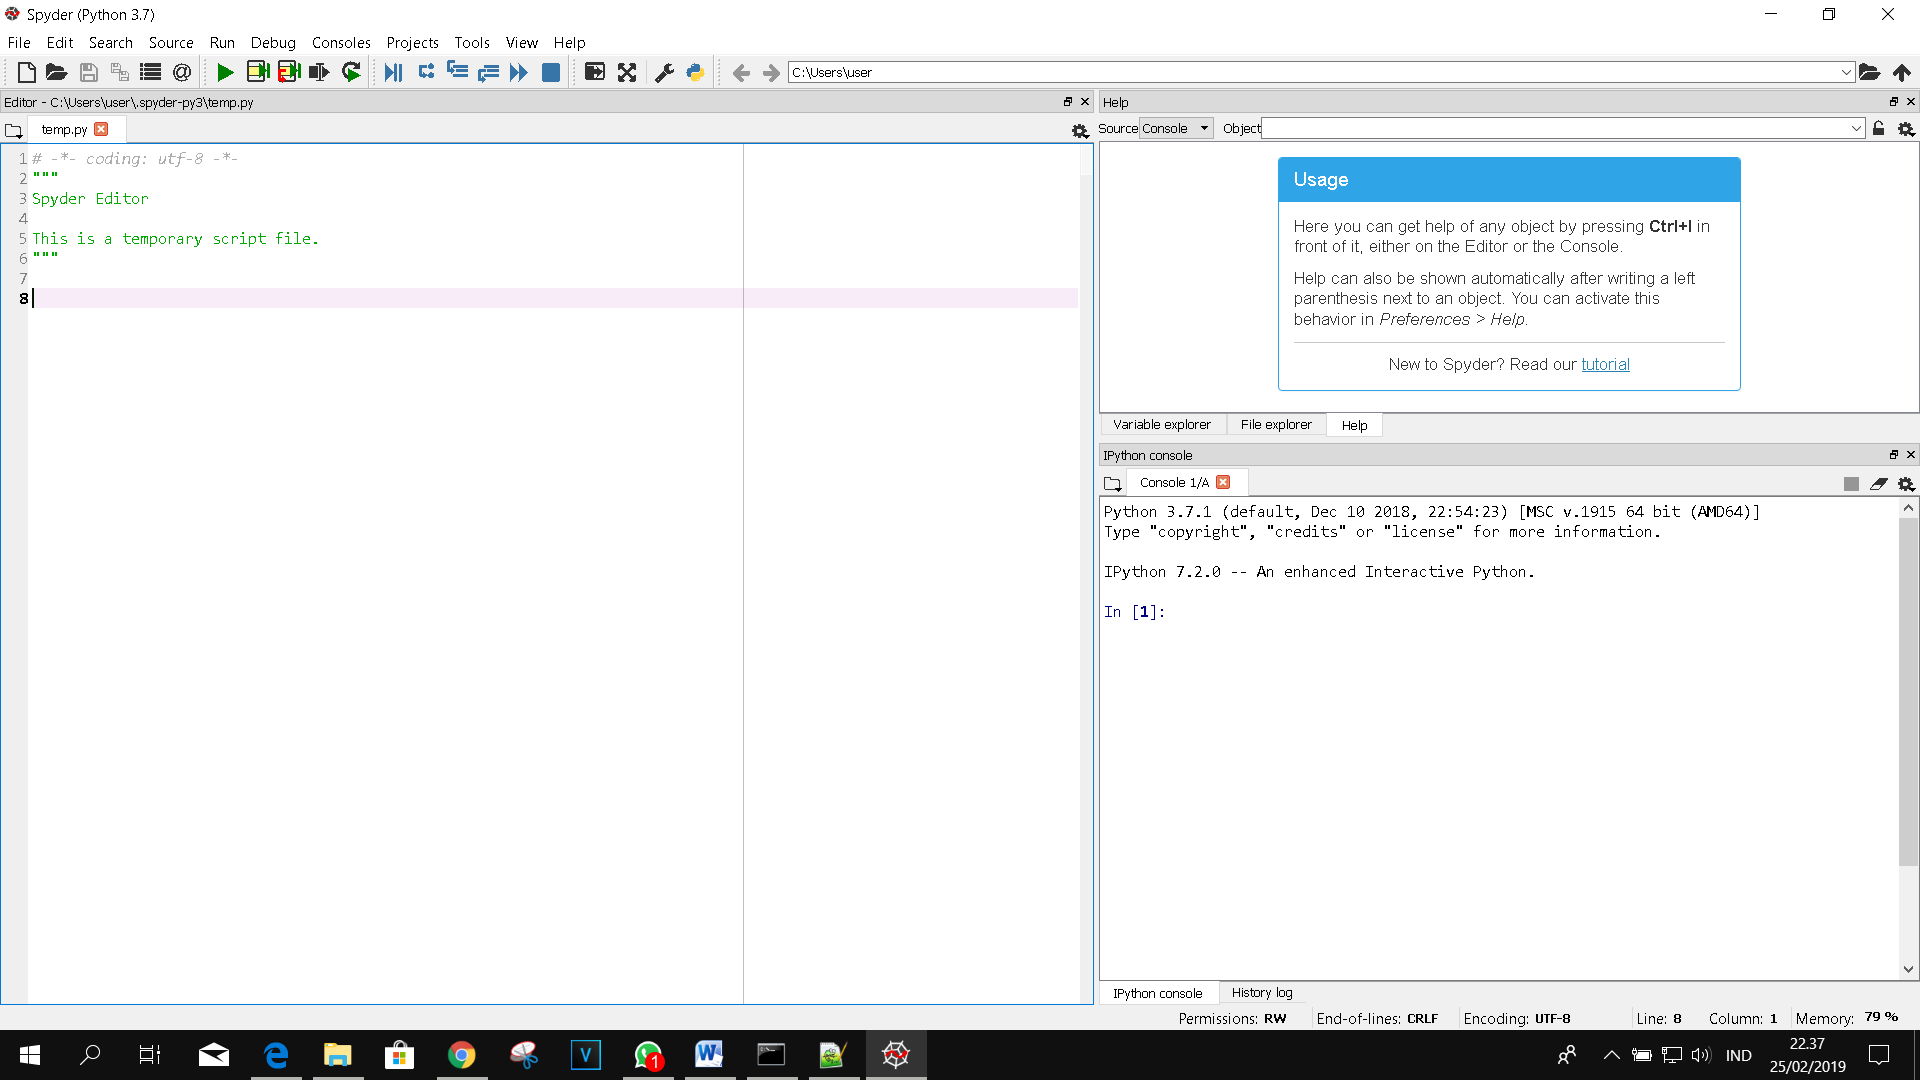
\includegraphics[width=10cm]{figures/fahmi/3.png}
		\centering
	\end{figure}
